\documentclass{standalone} 
\usepackage{tikz}
\usepackage{pgfplots}
\pgfplotsset{
  label style = {font=\sansmath\sffamily\small}
}
\begin{document}
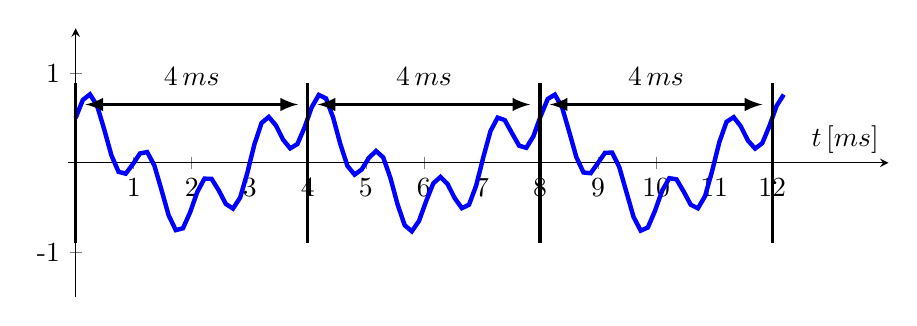
\begin{tikzpicture}

\begin{axis}[
    width=12cm, height=5cm,
    axis x line=center, 
    axis y line=middle, 
    samples=100,
    ymin=-3, ymax=3,
    xmin=-0.2, xmax=22,
    domain=0*pi:6.1*pi,
    ytick={-2,2},
    yticklabels={-1,1},
    xtick={        
        1.5708, 3.14159, 4.7123889, 6.28318, 7.85398, 9.424778,
        10.99557, 12.56637, 14.137167, 15.70796, 17.27876, 18.84955
    },
    xticklabels={
        $1$, $2$, $3$, $4$,
        $5$, $6$, $7$, $8$, $9$, $10$, $11$, $12$
    },
    xlabel={$t\,[ms]$}
]
\addplot [mark=none, ultra thick, blue] {cos(deg(x)) +
  0.6*sin(deg(4*x))};

\node (source) at (axis cs:0,1.3){};
\node (destination) at (axis cs:6.28318,1.3){};
\draw[very thick,<->, >=latex](source)--(destination); 
\node[above] (text) at (axis cs:3.1415,1.5) {$4\,ms$};

\node (or1) at (axis cs:0,2){};
\node (or2) at (axis cs:0,-2){};
\draw[very thick, -](or1)--(or2);

\node (neg1) at (axis cs:6.28318,2){};
\node (neg2) at (axis cs:6.28318,-2){};
\draw[very thick, -](neg1)--(neg2);

\node (pos1) at (axis cs:12.56637,2){};
\node (pos2) at (axis cs:12.56637,-2){};
\draw[very thick, -](pos1)--(pos2);

\node (source2) at (axis cs:6.28318,1.3){};
\node (destination2) at (axis cs:12.56637,1.3){};
\draw[very thick,<->, >=latex](source2)--(destination2); 
\node[above] (text) at (axis cs:9.424778,1.5) {$4\,ms$};

\node (pos3) at (axis cs:18.84955,2){};
\node (pos4) at (axis cs:18.84955,-2){};
\draw[very thick, -](pos3)--(pos4);

\node (source3) at (axis cs:12.56637,1.3){};
\node (destination3) at (axis cs:18.84955,1.3){};
\draw[very thick,<->, >=latex](source3)--(destination3); 
\node[above] (text) at (axis cs:15.70796,1.5) {$4\,ms$};

\end{axis}


\end{tikzpicture}
 

\end{document}